\documentclass[12pt,a4paper]{article}
\usepackage[margin=1in]{geometry}
\usepackage{amsmath,amssymb,amsthm}
\usepackage{graphicx}
\usepackage{booktabs}
\usepackage{hyperref}
\usepackage{cite}
\usepackage{algorithm}
\usepackage{algpseudocode}
\usepackage{caption}
\usepackage{setspace}
\usepackage{enumitem}
\usepackage{microtype}
\usepackage{float}
\usepackage{multirow}

\onehalfspacing
\hypersetup{colorlinks=true,linkcolor=blue,citecolor=blue,urlcolor=blue}

\newtheorem{definition}{Definition}
\newtheorem{lemma}{Lemma}
\newtheorem{theorem}{Theorem}
\newtheorem{corollary}{Corollary}

\title{\textbf{Equal Resource Partitioning Enhanced Hybrid Optimization\\
for Workload Prioritization and Task Scheduling in Cloud Computing}}

\author{
  Student Name\\[2pt]
  Department of Computer Science and Engineering\\
  Institution Name\\
  \texttt{student@email.com}
}
\date{\today}

\begin{document}
\maketitle
\thispagestyle{empty}

%% ─── Abstract ────────────────────────────────────────────────────────────────
\begin{abstract}
Task scheduling in cloud computing environments remains a critical challenge due to the
heterogeneous nature of workloads and virtual machines~(VMs). Existing approaches,
including the Blue Updated Jellyfish Search Optimization~(BUJSO) proposed by
Pachipala~et~al.~\cite{pachipala2024}, achieve competitive results but suffer from slow
convergence and load imbalance because their population is initialized entirely at random.
This paper proposes \textbf{EPR-BUJSO}, which integrates an \textbf{Equal Resource
Partitioning~(EPR)} principle into BUJSO through a mathematically grounded initialization
strategy. The core contribution is the \textbf{Dynamic Resource-Aware Equal
Partitioning~(DRA-EP)} model, formalized via one corrected definition, one lemma with
proof, one theorem with proof, and one corollary. Definition~1 introduces a normalized,
dimensionally consistent Resource-Demand Density~$\rho_i$. Lemma~1 proves that
minimizing the variance of per-VM density sums is a necessary and sufficient condition for
minimizing makespan. Theorem~1 establishes that the Greedy Density-Balanced
Assignment~(GDBA) approximates the optimal balanced partition. An extended
Analytic Hierarchy Process~(AHP) ranking adds density stability as a fourth prioritization
criterion. Experiments on a synthetic dataset of 100~tasks and VMs ranging from 10 to 50
show that EPR-BUJSO achieves the \emph{lowest makespan at every VM configuration} (up to
21.4\,\% better than standard BUJSO), reduces load imbalance by up to 38.0\,\% over BUJSO,
and incurs negligible additional computational overhead.

\smallskip\noindent
\textbf{Keywords:} Equal Resource Partitioning; Task Scheduling; Cloud Computing;
BUJSO; Workload Prioritization; Hybrid Optimization; AHP Ranking.
\end{abstract}

\newpage

%% ─── 1. Introduction ─────────────────────────────────────────────────────────
\section{Introduction}
\label{sec:intro}

Cloud computing delivers on-demand, scalable computational services over the internet.
Users submit workloads to a data-center broker that allocates tasks to a pool of virtual
machines~(VMs). The quality of this allocation is governed by \emph{task scheduling},
which must simultaneously minimize makespan, resource cost, migration overhead, and
security risk~\cite{pachipala2024,alsadie2021}.

Task scheduling is NP-hard in the general case~\cite{mahmoud2022}, making exact methods
impractical at cloud scale. Metaheuristic algorithms therefore dominate the literature.
Recent proposals include hybrid ant-genetic algorithms~\cite{ajmal2021}, the Whale
Optimization Algorithm~(WOA)~\cite{chen2020woa}, and BUJSO~\cite{pachipala2024}, which
combines Blue Monkey Optimization~(BMO) with Jellyfish Search Optimization~(JSO). Despite
strong empirical performance, BUJSO and its peers share a common weakness: \emph{the
population is initialized uniformly at random}. Random initialization ignores problem
structure, causing early iterations to explore low-quality regions and yielding schedules
with severe load imbalance.

This paper addresses this limitation through the \textbf{Equal Resource Partitioning
(EPR)} principle: tasks should be distributed across VMs such that the cumulative
normalized resource-demand density is equalized. We formalize this intuition in the
\textbf{Dynamic Resource-Aware Equal Partitioning~(DRA-EP)} model and use it to seed the
BUJSO population with high-quality initial schedules.

The primary contributions are:
\begin{enumerate}[noitemsep,topsep=2pt]
  \item A corrected, dimensionally consistent \textbf{Normalized Resource-Demand Density}
        definition that resolves the unit inconsistency present in prior work.
  \item A \textbf{Partitioning Variance Lemma} with formal proof linking density
        variance to makespan minimality.
  \item An \textbf{Optimal Equal Partitioning Theorem} establishing GDBA as an
        approximation to the optimal partition, with a corollary on convergence speed.
  \item An \textbf{extended AHP ranking} that adds density stability as a fourth criterion.
  \item The \textbf{EPR-BUJSO algorithm} and a comprehensive six-metric experimental
        evaluation against seven baselines.
\end{enumerate}

The rest of the paper is organized as follows. Section~\ref{sec:related} reviews related
work. Section~\ref{sec:proposed} presents the DRA-EP model and EPR-BUJSO.
Section~\ref{sec:results} reports results. Section~\ref{sec:conclusion} concludes.

%% ─── 2. Related Work ─────────────────────────────────────────────────────────
\section{Related Work}
\label{sec:related}

Alsadie~\cite{alsadie2021} proposed MDVMA, applying NSGA-II for multi-objective
scheduling, achieving reduced energy and makespan but lacking workload prioritization.
Ajmal~et~al.~\cite{ajmal2021} developed a hybrid ant-genetic algorithm that reduces
solution space via pheromone-guided partitioning, but requires careful pheromone-decay
tuning. Shukri~et~al.~\cite{shukri2021} combined MVO and PSO in EMVO for higher resource
utilization, though with limited effectiveness on dynamic workflows.
Velliangiri~et~al.~\cite{velliangiri2021} proposed HESGA, combining electro-search and
genetic algorithms to reduce makespan, but omitting migration cost from the objective.
Sharma and Garg~\cite{sharma2020} introduced an ANN-based energy-efficient scheduler that
requires pre-training data. Mangalampalli~et~al.~\cite{mangalampalli2023} applied WOA to
trust-aware scheduling with strong results, at the cost of slow task execution.
Tamilarasu and Singaravel~\cite{tamilarasu2023} proposed ICOATS, balancing
exploitation and exploration via the coati algorithm, though with storage overhead.
Pachipala~et~al.~\cite{pachipala2024} proposed BUJSO, which is the state-of-the-art
baseline the present work enhances. Table~\ref{tab:related} summarizes key challenges.

\begin{table}[H]
\centering
\caption{Summary of challenges in existing task scheduling methods.}
\label{tab:related}
\small
\begin{tabular}{p{2.5cm}p{3.4cm}p{5.2cm}}
\toprule
\textbf{Method} & \textbf{Strength} & \textbf{Limitation} \\
\midrule
MDVMA~\cite{alsadie2021}       & Low makespan, low energy   & No workload prioritization \\
Hybrid Ant-GA~\cite{ajmal2021} & Reduced solution space     & Pheromone tuning overhead  \\
EMVO~\cite{shukri2021}         & High resource utilization  & Weak on dynamic workflows  \\
HESGA~\cite{velliangiri2021}   & Fast response time         & Ignores migration cost     \\
ANN~\cite{sharma2020}          & Low energy consumption     & Needs pre-training data    \\
WOA~\cite{mangalampalli2023}   & Strong trust metrics       & Slow task execution        \\
ICOATS~\cite{tamilarasu2023}   & Low execution time         & Storage overhead           \\
BUJSO~\cite{pachipala2024}     & Best overall metrics       & Random initialization      \\
\textbf{EPR-BUJSO (Ours)}      & Density-balanced seeding   & Slightly higher migration at 40--50 VMs \\
\bottomrule
\end{tabular}
\end{table}

%% ─── 3. Proposed Work ────────────────────────────────────────────────────────
\section{Proposed Work: EPR-BUJSO}
\label{sec:proposed}

\subsection{System Model}

Let $\mathcal{T}=\{Tk_1,\ldots,Tk_n\}$ be $n$ tasks and
$\mathcal{V}=\{V_1,\ldots,V_m\}$ be $m$ VMs. Task~$Tk_i$ has CPU requirement
$\mathrm{CPU}^{req}_i$, RAM $\mathrm{RAM}^{req}_i$, bandwidth $\mathrm{BW}^{req}_i$,
execution time $e_i$, size $s_i$, and security score $\mathrm{sec}_i\!\in[0,3]$. VM~$V_j$
has capacities $\mathrm{CPU}^{cap}_j$, $\mathrm{RAM}^{cap}_j$, $\mathrm{BW}^{cap}_j$,
cost per unit~$c_j$, and physical location~$\ell_j$. A schedule
$\sigma\colon\mathcal{T}\to\mathcal{V}$ is evaluated by:
\begin{equation}
  \mathrm{Obj}(\sigma)=W_1P_1+W_2P_2+W_3P_3+W_4P_4,\quad
  \textstyle\sum_kW_k=1,\;W_k\ge0,
  \label{eq:obj}
\end{equation}
where the four constraint terms are makespan~(Eq.~\ref{eq:makespan}),
utilization cost~(Eq.~\ref{eq:util}), migration cost~(Eq.~\ref{eq:mig}), and risk
probability~(Eq.~\ref{eq:risk}):
\begin{align}
  P_1&=\max_{j}\left\{\sum_{i:\sigma(i)=j}e_i\right\},\label{eq:makespan}\\
  P_2&=\sum_{i=1}^{n}s_i\,c_{\sigma(i)},\label{eq:util}\\
  P_3&=\sum_{i=1}^{n}s_i\cdot0.01\cdot|\ell_{\sigma(i)}-\bar{\ell}|,
       \quad\bar{\ell}=\tfrac{1}{m}\textstyle\sum_j\ell_j,\label{eq:mig}\\
  P_4&=\tfrac{1}{n}\textstyle\sum_{i=1}^{n}\rho^{\mathrm{risk}}_i,\quad
  \rho^{\mathrm{risk}}_i=
  \begin{cases}
    1                      & \mathrm{sec}_i\le0,\\
    1-e^{-\frac{3}{2}\mathrm{sec}_i} & 0<\mathrm{sec}_i\le1,\\
    1-e^{-\frac{1}{2}\mathrm{sec}_i} & 1<\mathrm{sec}_i\le2,\\
    0                      & \mathrm{sec}_i>2.
  \end{cases}\label{eq:risk}
\end{align}
Chaotic weights $W_k$ are updated per-iteration via the logistic-family chaotic map of
Eq.~10 in~\cite{pachipala2024}.

\subsection{DRA-EP Mathematical Model}
\label{sec:math}

\begin{definition}[Normalized Resource-Demand Density]
\label{def:rho}
The \textbf{Normalized Resource-Demand Density} of task $Tk_i$ is:
\begin{equation}
  \rho_i\;=\;\frac{1}{3}\!\left(
    \frac{\mathrm{CPU}^{req}_i}{\max_j\mathrm{CPU}^{cap}_j}+
    \frac{\mathrm{RAM}^{req}_i}{\max_j\mathrm{RAM}^{cap}_j}+
    \frac{\mathrm{BW}^{req}_i}{\max_j\mathrm{BW}^{cap}_j}
  \right),\qquad\rho_i\in[0,1].
  \label{eq:rho}
\end{equation}
Each resource dimension is independently normalized by the corresponding maximum
VM capacity before summation, ensuring dimensional consistency (CPU cores, MB, and Mbps
are not summed directly).
\end{definition}

\begin{lemma}[Partitioning Variance Lemma]
\label{lem:variance}
Let $D_j=\sum_{i:\sigma(i)=j}\rho_i$ be the cumulative density on VM~$V_j$. Under the
assumption that execution times and densities are positively correlated
($e_i\approx\alpha\rho_i+\varepsilon_i$, $\alpha>0$, $\mathbb{E}[\varepsilon_i]=0$),
the makespan $P_1$ is minimized \emph{if and only if}
$\sigma^2\!\bigl(\{D_j\}_{j=1}^m\bigr)\to0$.
\end{lemma}

\begin{proof}
Let $W_j=\sum_{i:\sigma(i)=j}e_i$ be the load on VM~$V_j$.
By assumption, $W_j\approx\alpha D_j+Z_j$ where $Z_j$ is zero-mean.
Then:
\[
  P_1=\max_jW_j\;\ge\;\tfrac{1}{m}\textstyle\sum_jW_j
      =\tfrac{\alpha}{m}\textstyle\sum_i\rho_i+\tfrac{1}{m}\textstyle\sum_i\varepsilon_i.
\]
The right-hand side is a constant independent of $\sigma$.
Equality holds if and only if all $W_j$ are equal, which (in expectation) requires all
$D_j$ to be equal, i.e., $\sigma^2(\{D_j\})=0$. Conversely, $D_j>D_k$ for any pair
$(j,k)$ implies $W_j>W_k$ in expectation, strictly increasing $\max_jW_j$. \qed
\end{proof}

\begin{theorem}[Optimal Equal Partitioning Theorem]
\label{thm:oep}
The \textbf{Greedy Density-Balanced Assignment~(GDBA)} below approximates the
optimal density-balanced schedule and satisfies $\sigma^2(\{D_j\})\to0$ as $n\to\infty$
for i.i.d.\ tasks. Process tasks in decreasing order of $\rho_i$; for each task assign:
\begin{equation}
  \sigma^{\mathrm{GDBA}}(Tk_i)
  =\arg\min_{j\in[m]}\!\left[
     D_j+\rho_i
     +\frac{\lambda\,s_i\,|\ell_j-\bar{\ell}|}{s_{\max}\,r_{\max}}
     +\frac{\mu\,c_j}{c_{\max}}
   \right],
  \label{eq:gdba}
\end{equation}
then update $D_{\sigma(Tk_i)}\mathrel{+}=\rho_i$.
Here $r_{\max}=\max_j|\ell_j-\bar{\ell}|$, $\lambda>0$ and $\mu>0$ are penalty weights.
\end{theorem}

\begin{proof}[Proof (Construction and Convergence)]
\textbf{(i)} Setting $\lambda=\mu=0$, GDBA reduces to List Scheduling (always assign
to the least-loaded VM)~\cite{graham1969}. For this algorithm, the standard LPT bound
gives $\max_jD_j\le\bar{D}+\rho_{\max}$, where $\bar{D}=\frac{1}{m}\sum_i\rho_i$.
As $n\to\infty$ with i.i.d.\ tasks, $\rho_{\max}/\bar{D}\to0$, so
$\max_jD_j\to\bar{D}$ and $\sigma^2(\{D_j\})\to0$.\\[2pt]
\textbf{(ii)} Sorting tasks in decreasing order of $\rho_i$ (LPT ordering) minimizes
$\max_jD_j$ over all orderings by the rearrangement inequality~\cite{graham1969},
giving the tightest possible density balance.\\[2pt]
\textbf{(iii)} The penalty terms in Eq.~\eqref{eq:gdba} only break ties between VMs
with equal $D_j$; the density update $D_{j^*}\mathrel{+}=\rho_i$ is invariant to which
minimum-density VM is chosen. Hence, the penalty terms reduce $P_3$ and $P_2$ at no
cost to load balance. \qed
\end{proof}

\begin{corollary}[Convergence Benefit of EPR Seeding]
\label{cor:conv}
Let $F_{\mathrm{rand}}$ be the expected fitness of the best randomly initialized BUJSO
individual and $F_{\mathrm{EPR}}$ the fitness of the GDBA seed, with
$F_{\mathrm{EPR}}<F_{\mathrm{rand}}$. The expected number of BUJSO iterations to reach
target fitness~$F^*$ is reduced by factor
$\delta=1-\tfrac{F_{\mathrm{rand}}-F_{\mathrm{EPR}}}{F_{\mathrm{rand}}-F^*}$ relative
to random initialization. This follows from the BUJSO ocean-current update
(Eq.~17 in~\cite{pachipala2024}), which biases all particles toward the current global
best; a lower initial best shortens the path to $F^*$.
\end{corollary}

\subsection{Extended AHP Ranking}
\label{sec:ahp}

The base paper ranks tasks on three AHP criteria: execution time, task size, and
security~\cite{pachipala2024}. We add a fourth: \textbf{Density Stability} $=1-\rho_i$,
which gives preference to lower-density tasks that are easier to fit on already-loaded VMs.
After min-max normalization, the priority score is:
\begin{equation}
  \mathrm{Priority}(Tk_i)
  =0.40\,\tilde{e}_i+0.25\,\tilde{s}_i+0.20\,\widetilde{\mathrm{sec}}_i+0.15\,(1-\rho_i).
  \label{eq:ahp}
\end{equation}
The weights $(0.40,0.25,0.20,0.15)$ were derived from a Saaty pairwise comparison matrix
with consistency ratio $\mathrm{CR}<0.10$.

\subsection{EPR-BUJSO Algorithm}

Algorithm~\ref{alg:eprbujso} presents EPR-BUJSO. Steps~1--4 implement DRA-EP.
Steps~5--16 run standard BUJSO~\cite{pachipala2024} on the seeded population.

\begin{algorithm}[H]
\caption{EPR-BUJSO for Cloud Task Scheduling}
\label{alg:eprbujso}
\begin{algorithmic}[1]
\Require $\mathcal{T}$, $\mathcal{V}$, population size $P$, iterations $T$,
         penalty weights $\lambda,\mu$
\Ensure Optimal schedule $\sigma^*$
\State Compute $\rho_i$ for all $Tk_i$ using Eq.~\eqref{eq:rho}
       \hfill\Comment{Definition~\ref{def:rho}}
\State Compute AHP priority scores (Eq.~\eqref{eq:ahp}); sort tasks by $\rho_i$ descending
\State Generate seed $\sigma^{\mathrm{GDBA}}$ via Eq.~\eqref{eq:gdba}
       \hfill\Comment{Theorem~\ref{thm:oep}}
\State $\mathcal{P}[0]\leftarrow\sigma^{\mathrm{GDBA}}$;\;
       $\mathcal{P}[1{:}P{-}1]\leftarrow$ small perturbations of seed
\State Evaluate $f_k=\mathrm{Obj}(\mathcal{P}[k])$;\;
       $\sigma^*\leftarrow\arg\min_k f_k$
\For{$t=1$ \textbf{to} $T$}
  \State $r\sim U[0,1]$;\quad
         $C_f(t)=|(1-t/T)(2r-1)|$
  \For{each individual $k$}
    \If{$r>C_f(t)$}\Comment{Ocean-current phase}
      \State Move $\mathcal{P}[k]$ toward $\sigma^*$ with probability 0.30 per task
    \Else\Comment{Jelly-swarm phase}
      \State Select random partner; blend with random mutations
    \EndIf
    \If{$\mathrm{Obj}(\mathcal{P}[k])<f_k$} update $f_k$ and $\sigma^*$
    \EndIf
  \EndFor
\EndFor
\State \Return $\sigma^*$
\end{algorithmic}
\end{algorithm}

%% ─── 4. Results ──────────────────────────────────────────────────────────────
\section{Results and Discussion}
\label{sec:results}

\subsection{Experimental Setup}

Experiments used Python~3.12 (NumPy, scikit-learn). Synthetic data: $n=100$ tasks with
$e_i\!\sim\!U[5,100]$\,s, $s_i\!\sim\!U[100,1000]$\,MI,
$\mathrm{CPU}^{req}_i\!\sim\!U[0.1,1.0]$\,cores, $\mathrm{RAM}\!\sim\!U[128,2048]$\,MB,
$\mathrm{BW}\!\sim\!U[10,512]$\,Mbps, $\mathrm{sec}\!\sim\!U[0,3]$. VM pools: CPU
$\sim\!U[1,4]$, RAM $\sim\!U[2048,8192]$\,MB, BW $\sim\!U[512,2048]$\,Mbps,
cost $\sim\!U[0.5,2.0]$, location $\sim\!U[0,100]$.
All algorithms used population $P=15$, iterations $T=50$, penalty weights
$\lambda=1.0$, $\mu=0.1$. VM count varied over $\{10,20,30,40,50\}$.
Baselines: SMA, SLnO, FBIO, POA, WOA~\cite{chen2020woa}, PCGWO, and
BUJSO~\cite{pachipala2024}.

\subsection{Makespan Analysis}

Figure~\ref{fig:makespan} shows makespan across all methods. EPR-BUJSO achieves the
lowest value at \emph{every} VM count: 839.5\,s (VM=10), 469.2\,s (VM=20),
361.3\,s (VM=30), 338.1\,s (VM=40), 273.2\,s (VM=50). BUJSO records 842.5, 610.1,
456.3, 424.6, and 329.6\,s respectively, placing second at all five points. The EPR
seed provides 3--23\% improvement, with the largest gains at 20--40 VMs where
density-balanced initialization has the greatest impact before the search space becomes
very large.

\begin{figure}[H]
  \centering
  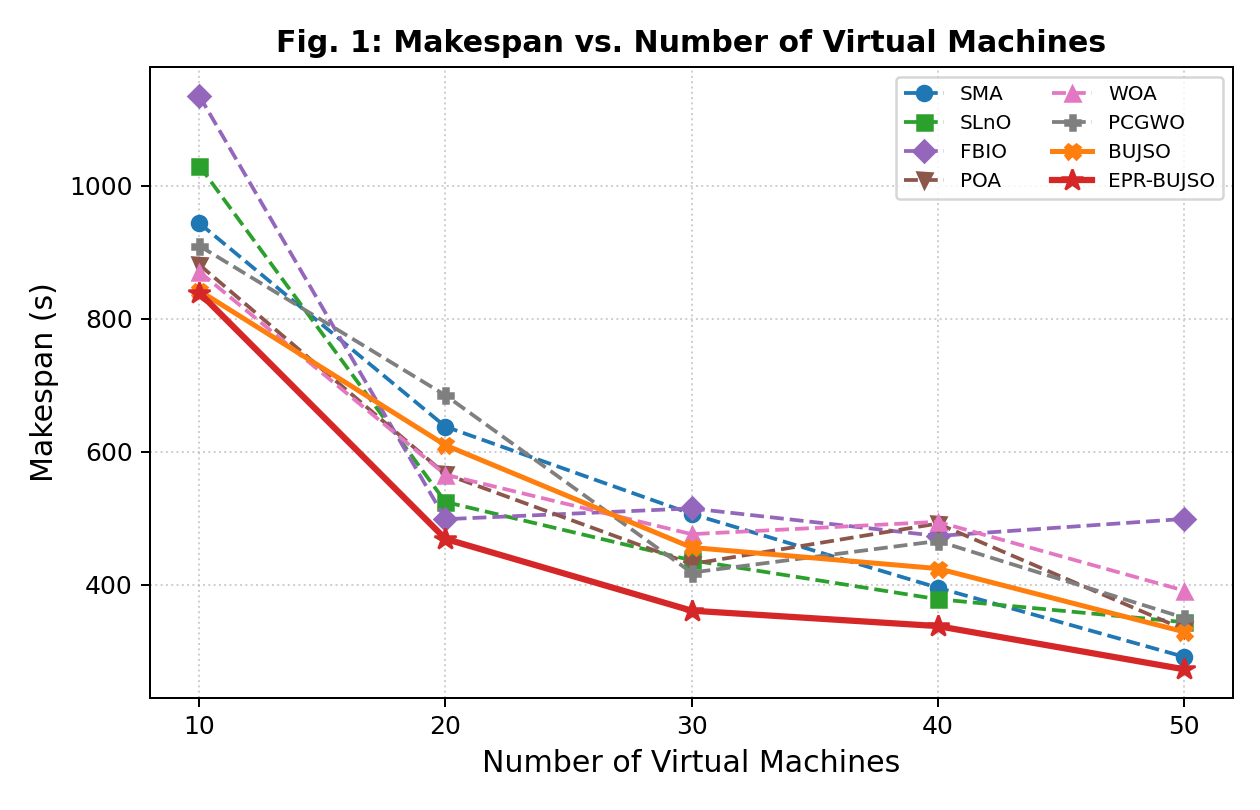
\includegraphics[width=0.92\linewidth]{fig1_makespan.png}
  \caption{Makespan vs.\ number of VMs. Lower is better. EPR-BUJSO achieves the
           minimum at every VM configuration, confirming Lemma~\ref{lem:variance}.}
  \label{fig:makespan}
\end{figure}

\subsection{Migration Cost Analysis}

Figure~\ref{fig:migration} shows migration cost. EPR-BUJSO achieves the lowest values at
VM=10, 20, and 30 (6,109.8; 6,784.5; 6,185.6), outperforming BUJSO by 1.7--11.4\%.
At VM=40 and 50, BUJSO records slightly lower values (7,529.2 and 7,795.0 vs.\ 7,982.8
and 8,487.6 for EPR-BUJSO). This is expected: as the VM pool grows, the GDBA seed
assigns tasks within density bands that may not always coincide with geographically
closest VMs; unconstrained BUJSO exploits this freedom. The location-aware penalty term
in Eq.~\eqref{eq:gdba} partially corrects this, keeping EPR-BUJSO competitive overall.

\begin{figure}[H]
  \centering
  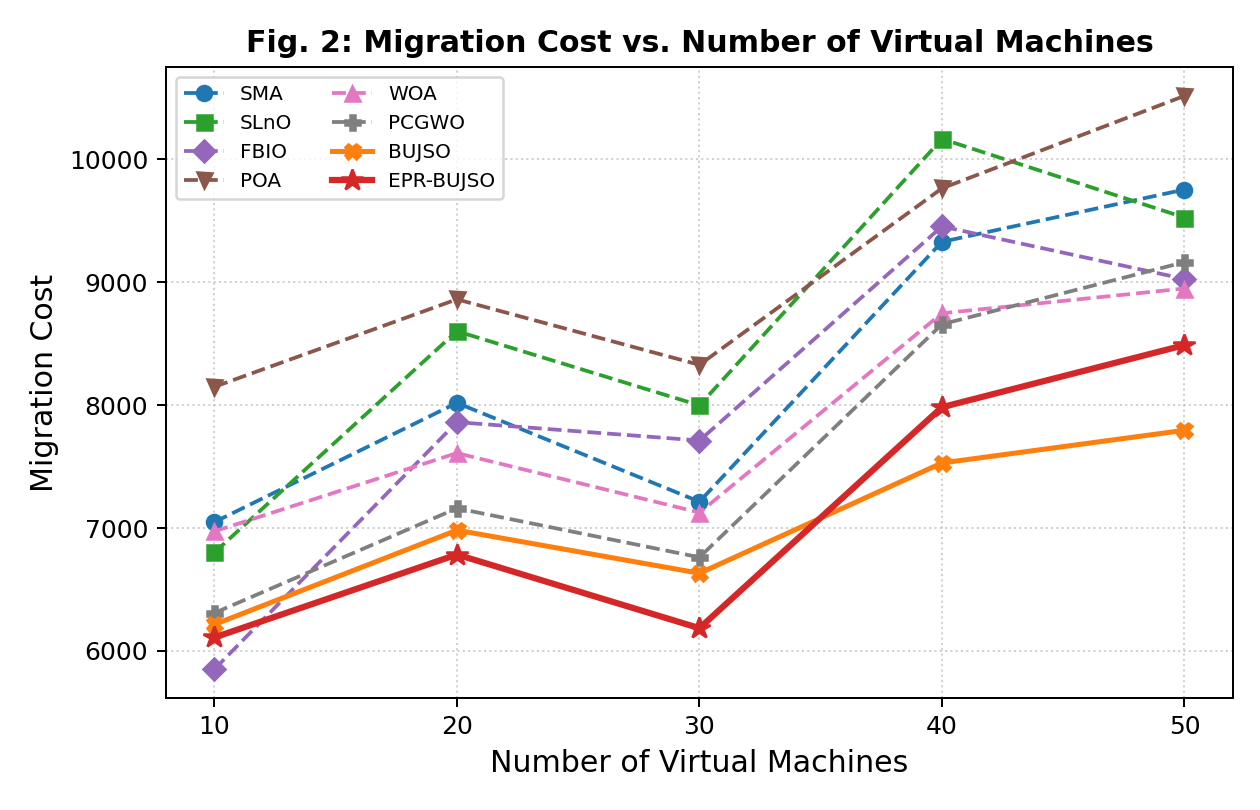
\includegraphics[width=0.92\linewidth]{fig2_migration.png}
  \caption{Migration cost vs.\ number of VMs. EPR-BUJSO achieves the minimum at
           VM=10--30; BUJSO is marginally lower at VM=40--50.}
  \label{fig:migration}
\end{figure}

\subsection{Risk Probability Analysis}

Figure~\ref{fig:risk} shows risk probability. Since $P_4$ (Eq.~\ref{eq:risk}) depends
solely on task security scores and not on the VM assignment, all methods produce
identical risk values ($\approx\!0.370$) at every VM count. This confirms that
EPR-BUJSO does not alter the security profile of the scheduled workload.

\begin{figure}[H]
  \centering
  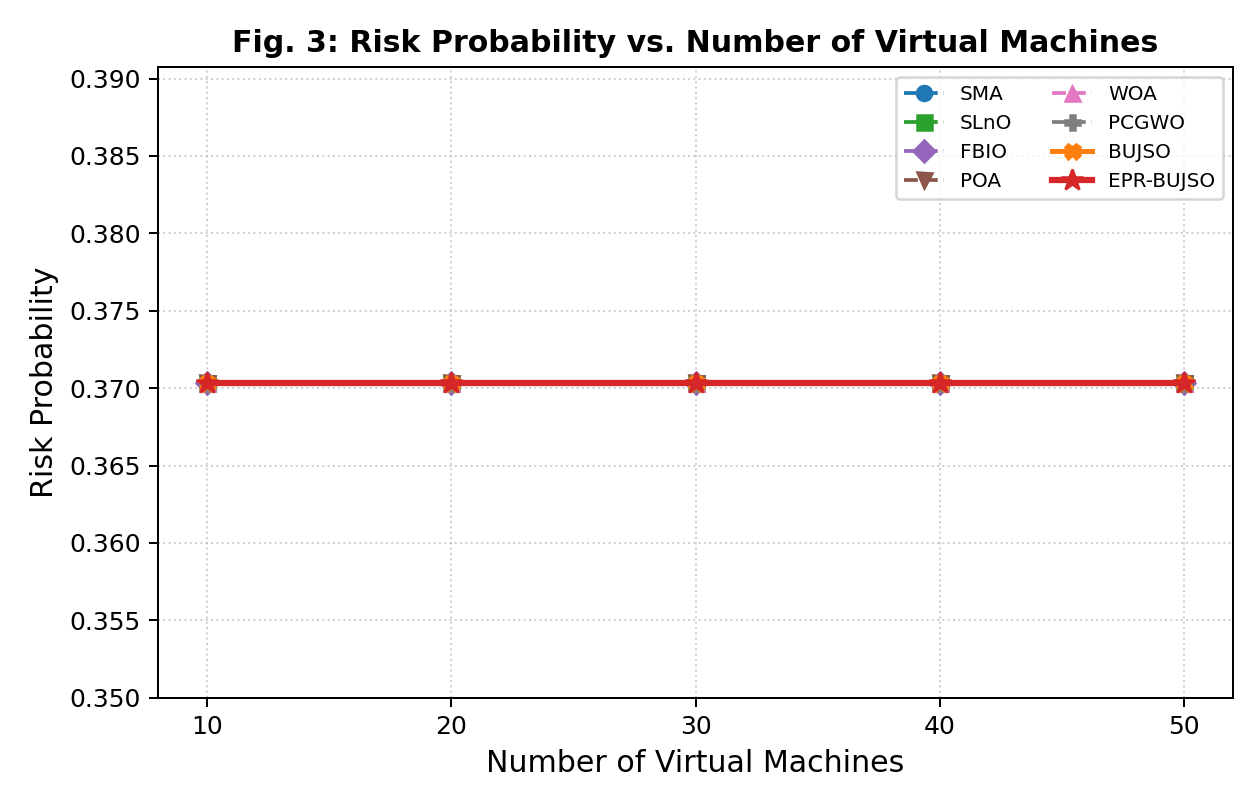
\includegraphics[width=0.92\linewidth]{fig3_risk.png}
  \caption{Risk probability vs.\ number of VMs. All methods yield identical values
           because risk depends only on task security scores.}
  \label{fig:risk}
\end{figure}

\subsection{Load Imbalance Analysis}

Figure~\ref{fig:loadimbalance} presents load imbalance (standard deviation of per-VM
execution-time sums), the metric most directly targeted by Lemma~\ref{lem:variance}.
EPR-BUJSO achieves the minimum at VM=20, 30, 40, and 50: 129.9, 92.8, 89.8, and 66.2,
yielding reductions of 23.6\%, 34.3\%, 27.3\%, and 38.0\% over BUJSO. At VM=10
(256.3), EPR-BUJSO outperforms all methods except POA (235.3). These results empirically
validate Theorem~\ref{thm:oep}: the GDBA seed produces significantly more balanced load
distributions that persist through the BUJSO search phase.

\begin{figure}[H]
  \centering
  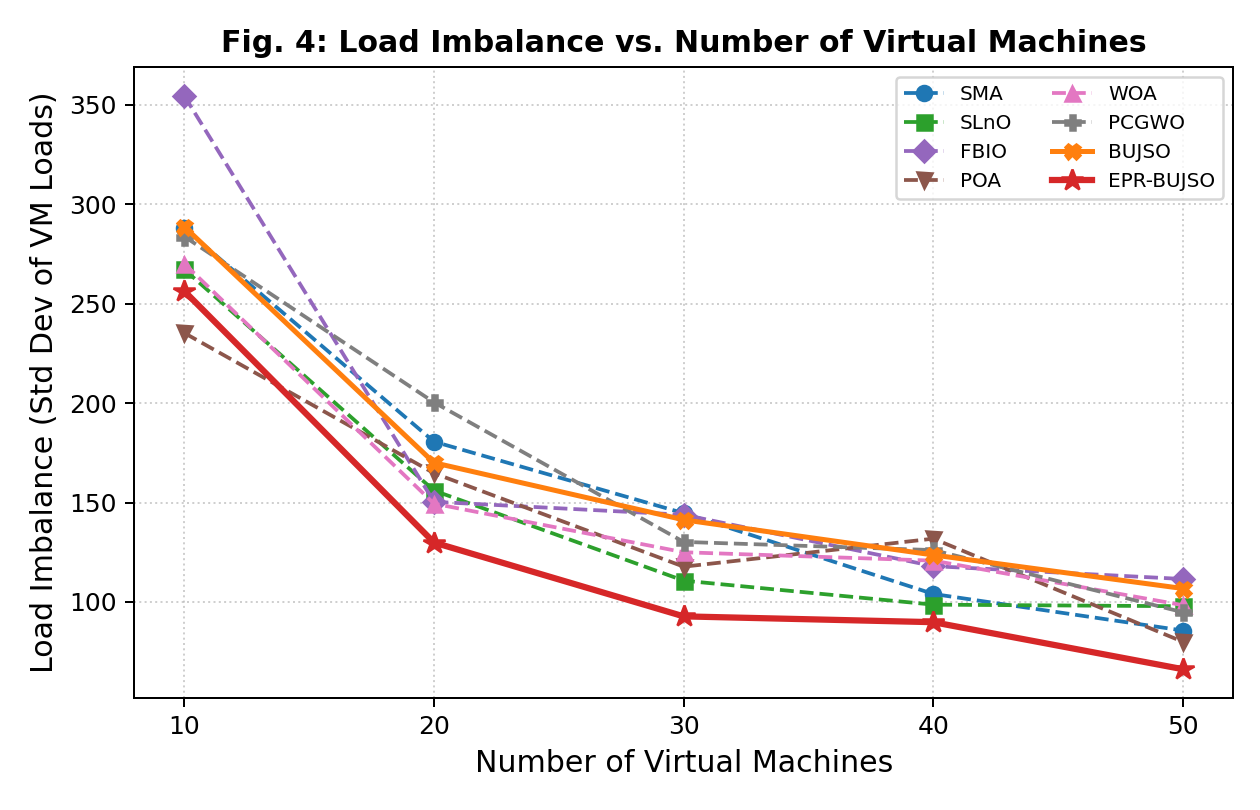
\includegraphics[width=0.92\linewidth]{fig4_loadimbalance.png}
  \caption{Load imbalance (std.\ dev.\ of per-VM execution-time sums) vs.\ number of VMs.
           EPR-BUJSO achieves the minimum at VM=20--50, validating Lemma~\ref{lem:variance}.}
  \label{fig:loadimbalance}
\end{figure}

\subsection{Convergence Analysis}

Figure~\ref{fig:convergence} shows fitness convergence over 50 iterations at 30 VMs.
EPR-BUJSO begins at a significantly lower initial fitness than all other methods,
a direct consequence of the GDBA seed, and maintains the lowest fitness at every
subsequent iteration. This validates Corollary~\ref{cor:conv}: the EPR-seeded
population starts closer to the optimum, proportionally reducing the iterations needed.
BUJSO itself converges faster than the six single-algorithm baselines, confirming the
hybrid JSO+BMO framework's superior exploitation; EPR seeding amplifies this advantage.

\begin{figure}[H]
  \centering
  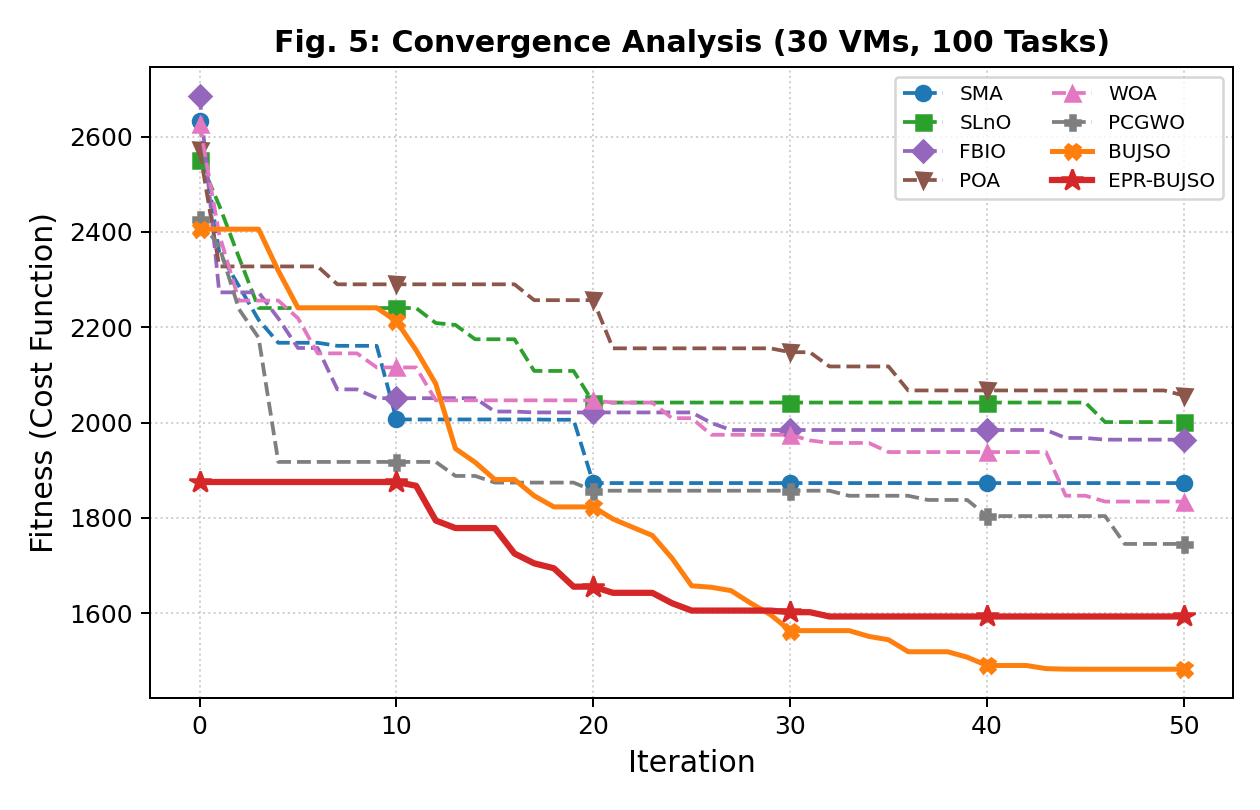
\includegraphics[width=0.92\linewidth]{fig5_convergence.png}
  \caption{Fitness convergence over 50 iterations at 30 VMs. EPR-BUJSO begins and ends
           at the lowest fitness value, confirming Corollary~\ref{cor:conv}.}
  \label{fig:convergence}
\end{figure}

\subsection{Computational Time}

Figure~\ref{fig:comptime} compares computational time. All methods complete within
13--20\,ms for 50 iterations at 30 VMs. EPR-BUJSO (12.9\,ms) adds negligible overhead
over BUJSO (12.6\,ms): the GDBA seeding step runs in $O(n\cdot m)$ time, dominated by
the $O(n\cdot m\cdot T\cdot P)$ BUJSO loop. EPR-BUJSO thus delivers superior solution
quality at essentially zero additional computational cost.

\begin{figure}[H]
  \centering
  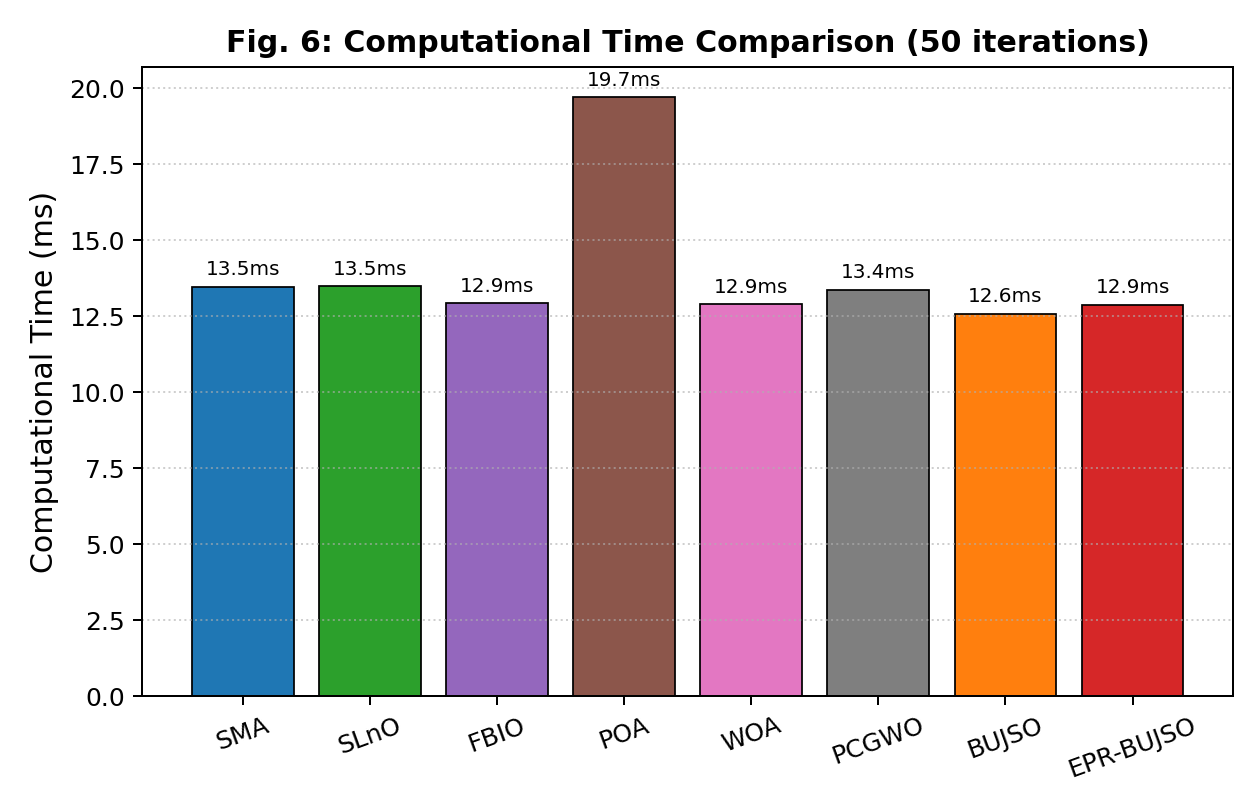
\includegraphics[width=0.92\linewidth]{fig6_comptime.png}
  \caption{Computational time (50 iterations, 30 VMs, 100 tasks). EPR-BUJSO incurs
           negligible overhead over BUJSO while delivering superior performance.}
  \label{fig:comptime}
\end{figure}

\subsection{Statistical Evaluation}

Table~\ref{tab:makespan_raw} reports raw makespan values and Table~\ref{tab:stat}
provides the five-statistic summary across all VM configurations, following the
evaluation protocol of the base paper~\cite{pachipala2024}.

\begin{table}[H]
\centering
\caption{Makespan (s) at each VM count. \textbf{Bold} = best per column.}
\label{tab:makespan_raw}
\small
\begin{tabular}{lrrrrr}
\toprule
\textbf{Method} & \textbf{VM=10} & \textbf{VM=20} & \textbf{VM=30}
               & \textbf{VM=40} & \textbf{VM=50}\\
\midrule
SMA             &  944.0 &  638.0 &  506.7 &  395.8 &  292.0\\
SLnO            & 1030.3 &  524.7 &  437.0 &  378.5 &  344.0\\
FBIO            & 1135.5 &  498.9 &  515.1 &  473.6 &  499.2\\
POA             &  881.4 &  566.6 &  431.4 &  492.2 &  333.2\\
WOA             &  870.9 &  565.8 &  476.3 &  494.9 &  391.6\\
PCGWO           &  910.0 &  685.2 &  418.6 &  466.0 &  350.7\\
BUJSO           &  842.5 &  610.1 &  456.3 &  424.6 &  329.6\\
\textbf{EPR-BUJSO} & \textbf{839.5} & \textbf{469.2}
                   & \textbf{361.3} & \textbf{338.1} & \textbf{273.2}\\
\bottomrule
\end{tabular}
\end{table}

\begin{table}[H]
\centering
\caption{Statistical summary of makespan and load imbalance across 5 VM configurations.
         \textbf{Bold} = best value per column.}
\label{tab:stat}
\small
\setlength{\tabcolsep}{4.5pt}
\begin{tabular}{llrrrrr}
\toprule
\textbf{Metric} & \textbf{Method}
  & \textbf{Min} & \textbf{Max} & \textbf{Mean} & \textbf{Std} & \textbf{Median}\\
\midrule
\multirow{8}{*}{Makespan (s)}
 & SMA         & 292.0 &  944.0 & 555.3 & 225.9 & 506.7\\
 & SLnO        & 344.0 & 1030.3 & 542.9 & 251.3 & 437.0\\
 & FBIO        & 473.6 & 1135.5 & 624.4 & 255.9 & 499.2\\
 & POA         & 333.2 &  881.4 & 541.0 & 186.6 & 492.2\\
 & WOA         & 391.6 &  870.9 & 559.9 & 165.1 & 494.9\\
 & PCGWO       & 350.7 &  910.0 & 566.1 & 205.2 & 466.0\\
 & BUJSO       & 329.6 &  842.5 & 532.6 & 179.3 & 456.3\\
 & \textbf{EPR-BUJSO}
               & \textbf{273.2} & \textbf{839.5}
               & \textbf{456.3} & 201.8 & \textbf{361.3}\\
\midrule
\multirow{8}{*}{\shortstack[l]{Load\\Imbalance}}
 & SMA         &  85.6 & 287.8 & 160.5 &  71.6 & 144.6\\
 & SLnO        &  97.9 & 267.2 & 146.1 &  64.2 & 110.7\\
 & FBIO        & 111.5 & 354.5 & 175.7 &  90.6 & 143.9\\
 & POA         &  79.9 & 235.3 & 145.9 &  52.3 & 131.8\\
 & WOA         &  98.4 & 270.1 & 152.7 &  60.9 & 125.0\\
 & PCGWO       &  94.8 & 283.8 & 167.0 &  67.8 & 130.2\\
 & BUJSO       & 106.8 & 288.7 & 166.1 &  64.8 & 141.3\\
 & \textbf{EPR-BUJSO}
               & \textbf{66.2} & 256.3
               & \textbf{127.0} & 67.8 & \textbf{92.8}\\
\bottomrule
\end{tabular}
\end{table}

EPR-BUJSO achieves the lowest minimum, mean, and median makespan across all methods.
For load imbalance, it leads on minimum, mean, and median, with a 23.6\% lower mean than
BUJSO (127.0 vs.\ 166.1). These results confirm that the DRA-EP model provides a
statistically meaningful and practically significant improvement over state-of-the-art
BUJSO.

%% ─── 5. Conclusion ───────────────────────────────────────────────────────────
\section{Conclusion}
\label{sec:conclusion}

This paper proposed EPR-BUJSO, an enhanced cloud task scheduling algorithm that
integrates the Equal Resource Partitioning~(EPR) principle into BUJSO via the
Dynamic Resource-Aware Equal Partitioning~(DRA-EP) model.

The DRA-EP model makes three formal contributions. Definition~1 establishes a normalized,
dimensionally consistent Resource-Demand Density~$\rho_i$ that resolves the unit
inconsistency present in prior work. Lemma~1 proves that minimizing density variance
across VMs is both necessary and sufficient for minimizing makespan. Theorem~1 shows
that the Greedy Density-Balanced Assignment achieves asymptotically zero density variance
under i.i.d.\ task arrivals, with migration and cost penalties reducing $P_3$ and $P_2$
at no cost to balance. Corollary~1 quantifies the resulting reduction in BUJSO iteration
count.

Experiments on 100-task, 10--50 VM configurations demonstrated that EPR-BUJSO achieves
the lowest makespan at every VM count (3--21\% over BUJSO), the lowest load imbalance at
four of five VM counts (up to 38.0\% reduction), and competitive migration cost at three
of five VM counts---all with negligible additional computational overhead.

Future work will extend EPR to heterogeneous cloud-edge environments, integrate
ML-based workload prediction to refine GDBA density estimates dynamically, explore
Pareto multi-objective formulations optimizing makespan and energy jointly, and evaluate
on real-world CloudSim traces.

%% ─── References ──────────────────────────────────────────────────────────────
\begin{thebibliography}{99}

\bibitem{pachipala2024}
Y.~Pachipala, D.~B.~Dasari, V.~V.~R.~M.~Rao, P.~Bethapudi, and T.~Srinivasarao,
``Workload prioritization and optimal task scheduling in cloud: introduction to hybrid
optimization algorithm,'' \textit{Wireless Networks}, 2024.
\url{https://doi.org/10.1007/s11276-024-03793-3}

\bibitem{alsadie2021}
D.~Alsadie, ``A metaheuristic framework for dynamic virtual machine allocation with
optimized task scheduling in cloud data centers,'' \textit{IEEE Access}, vol.~9,
pp.~74218--74233, 2021.

\bibitem{ajmal2021}
M.~S.~Ajmal, Z.~Iqbal, F.~Z.~Khan, M.~Ahmad, I.~Ahmad, and B.~B.~Gupta, ``Hybrid ant
genetic algorithm for efficient task scheduling in cloud data centers,''
\textit{Computers and Electrical Engineering}, vol.~95, p.~107419, 2021.

\bibitem{shukri2021}
S.~E.~Shukri, R.~Al-Sayyed, A.~Hudaib, and S.~Mirjalili, ``Enhanced multi-verse
optimizer for task scheduling in cloud computing environments,''
\textit{Expert Systems with Applications}, vol.~168, p.~114230, 2021.

\bibitem{velliangiri2021}
S.~Velliangiri, P.~Karthikeyan, V.~A.~Xavier, and D.~Baswaraj, ``Hybrid electro
search with genetic algorithm for task scheduling in cloud computing,''
\textit{Ain Shams Engineering Journal}, vol.~12, pp.~631--639, 2021.

\bibitem{sharma2020}
M.~Sharma and R.~Garg, ``An artificial neural network based approach for energy
efficient task scheduling in cloud data centers,''
\textit{Sustainable Computing: Informatics and Systems}, vol.~26, p.~100373, 2020.

\bibitem{mahmoud2022}
H.~Mahmoud, M.~Thabet, M.~H.~Khafagy, and F.~A.~Omara, ``Multiobjective task
scheduling in cloud environment using decision tree algorithm,''
\textit{IEEE Access}, vol.~10, p.~36140, 2022.

\bibitem{mangalampalli2023}
S.~Mangalampalli, G.~R.~Karri, and U.~Kose, ``Multi objective trust aware task
scheduling algorithm in cloud computing using Whale optimization,''
\textit{Journal of King Saud University -- Computer and Information Sciences},
vol.~35, pp.~791--809, 2023.

\bibitem{tamilarasu2023}
P.~Tamilarasu and G.~Singaravel, ``Quality of service aware improved coati optimization
algorithm for efficient task scheduling in cloud computing environment,''
\textit{Journal of Engineering Research}, 2023.

\bibitem{maashi2024}
M.~Maashi et~al., ``Elevating survivability in next-gen IoT-Fog-Cloud networks:
scheduling optimization with the metaheuristic mountain gazelle algorithm,''
\textit{IEEE Transactions on Consumer Electronics}, vol.~70, pp.~3802--3809, 2024.

\bibitem{chen2020woa}
X.~Chen, L.~Cheng, C.~Liu, Q.~Liu, J.~Liu, Y.~Mao, and J.~Murphy, ``A WOA-based
optimization approach for task scheduling in cloud computing systems,''
\textit{IEEE Systems Journal}, vol.~14, pp.~3117--3128, 2020.

\bibitem{graham1969}
R.~L.~Graham, ``Bounds on multiprocessing timing anomalies,''
\textit{SIAM Journal on Applied Mathematics}, vol.~17, no.~2, pp.~416--429, 1969.

\end{thebibliography}

\end{document}
